\documentclass[tikz,border=5pt]{standalone}
\usepackage[T1]{fontenc}
\usepackage{lmodern}
\usetikzlibrary{arrows.meta,positioning,fit}
\begin{document}
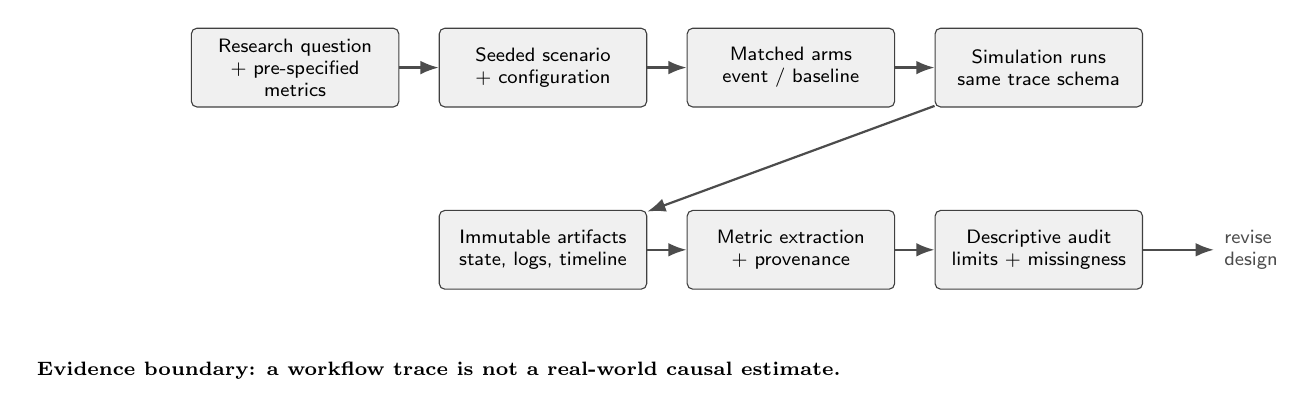
\begin{tikzpicture}[font=\sffamily\scriptsize,>=Latex,
 box/.style={draw=black!75,rounded corners=2pt,fill=black!6,text width=24mm,minimum height=10mm,align=center},
 flow/.style={->,thick,black!70}]
\node[box] (question) {Research question\\+ pre-specified metrics};
\node[box,right=5mm of question] (scenario) {Seeded scenario\\+ configuration};
\node[box,right=5mm of scenario] (arms) {Matched arms\\event / baseline};
\node[box,right=5mm of arms] (run) {Simulation runs\\same trace schema};
\draw[flow] (question) -- (scenario);
\draw[flow] (scenario) -- (arms);
\draw[flow] (arms) -- (run);

\node[box,below=13mm of scenario] (artifacts) {Immutable artifacts\\state, logs, timeline};
\node[box,below=13mm of arms] (extract) {Metric extraction\\+ provenance};
\node[box,below=13mm of run] (audit) {Descriptive audit\\limits + missingness};
\draw[flow] (run) -- (artifacts);
\draw[flow] (artifacts) -- (extract);
\draw[flow] (extract) -- (audit);
\draw[flow] (audit.east) -- ++(9mm,0) node[right,align=left]{revise\\design};
\node[font=\bfseries\scriptsize,anchor=west,below=8mm of artifacts.south west]
 {Evidence boundary: a workflow trace is not a real-world causal estimate.};
\end{tikzpicture}
\end{document}
